\documentclass{article}
\usepackage[utf8]{inputenc}
\usepackage{enumitem}
\usepackage{listings}
\usepackage{amsmath,amssymb}
\usepackage{geometry}
\usepackage[T1]{fontenc}
\usepackage{graphicx}


\geometry{
 a4paper,
 left=38mm,
 right=38mm,
 top=38mm,
 bottom=38mm
 }

\lstset{
    language=C,
    showstringspaces=false,
    breaklines=true
}



\title{ME 333 Final Project}
\author{Marshall Johnson}
\date{March 17, 2022}

\begin{document}

\maketitle

\section*{Homework 10}

\setcounter{section}{28}
\setcounter{subsection}{4}
\setcounter{subsubsection}{11}
\subsubsection{Trajectory Tracking}
\begin{enumerate}[label=\textbf{\arabic*})]
    \item \textbf{Turn in your best plots of following the step and cubic trajectories in Figure 28.5
    with the load attached. Indicate the control gains you used, as well as their units.} \\

        Ki = 100.0 \\
        Kd = 0.0 \\
        Kp = 1000.0 \\

        \textbf{Step} \\

        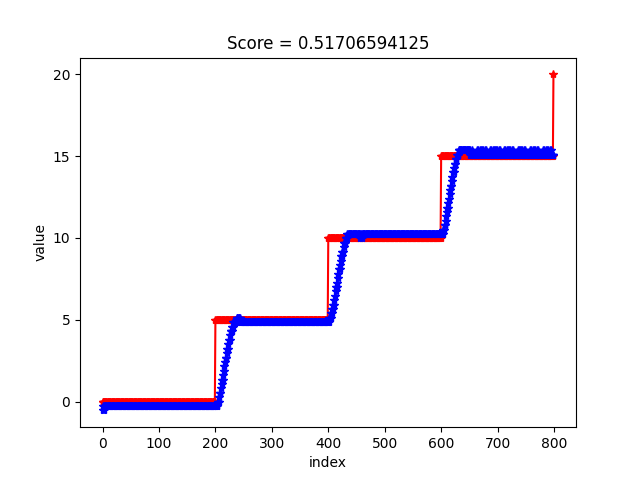
\includegraphics[width=\linewidth]{step.png}

        \pagebreak
        \textbf{Cubic} \\

        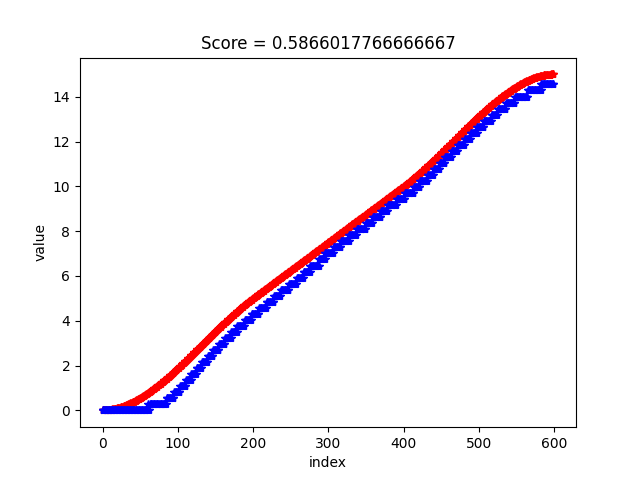
\includegraphics[width=\linewidth]{cubic.png}
\end{enumerate}



\end{document}
